\documentclass[tikz,border=5pt]{standalone}
\usepackage[T1]{fontenc}
\usepackage{lmodern,amsmath,amssymb}
\usetikzlibrary{arrows.meta,calc,positioning,fit,backgrounds,shapes.geometric,matrix,decorations.pathreplacing,patterns}
\definecolor{ink}{gray}{0.08}
\definecolor{wash}{gray}{0.965}
\definecolor{soft}{gray}{0.45}
\tikzset{box/.style={draw=ink,line width=.65pt,fill=white,align=center,inner sep=4pt,outer sep=0pt,font=\small},flow/.style={draw=ink,line width=.65pt,-{Latex[length=1.8mm,width=1.3mm]},rounded corners=2pt},annotation/.style={font=\scriptsize,text=soft,align=center},groupbox/.style={draw=soft,dashed,line width=.45pt,fill=wash}}
\begin{document}
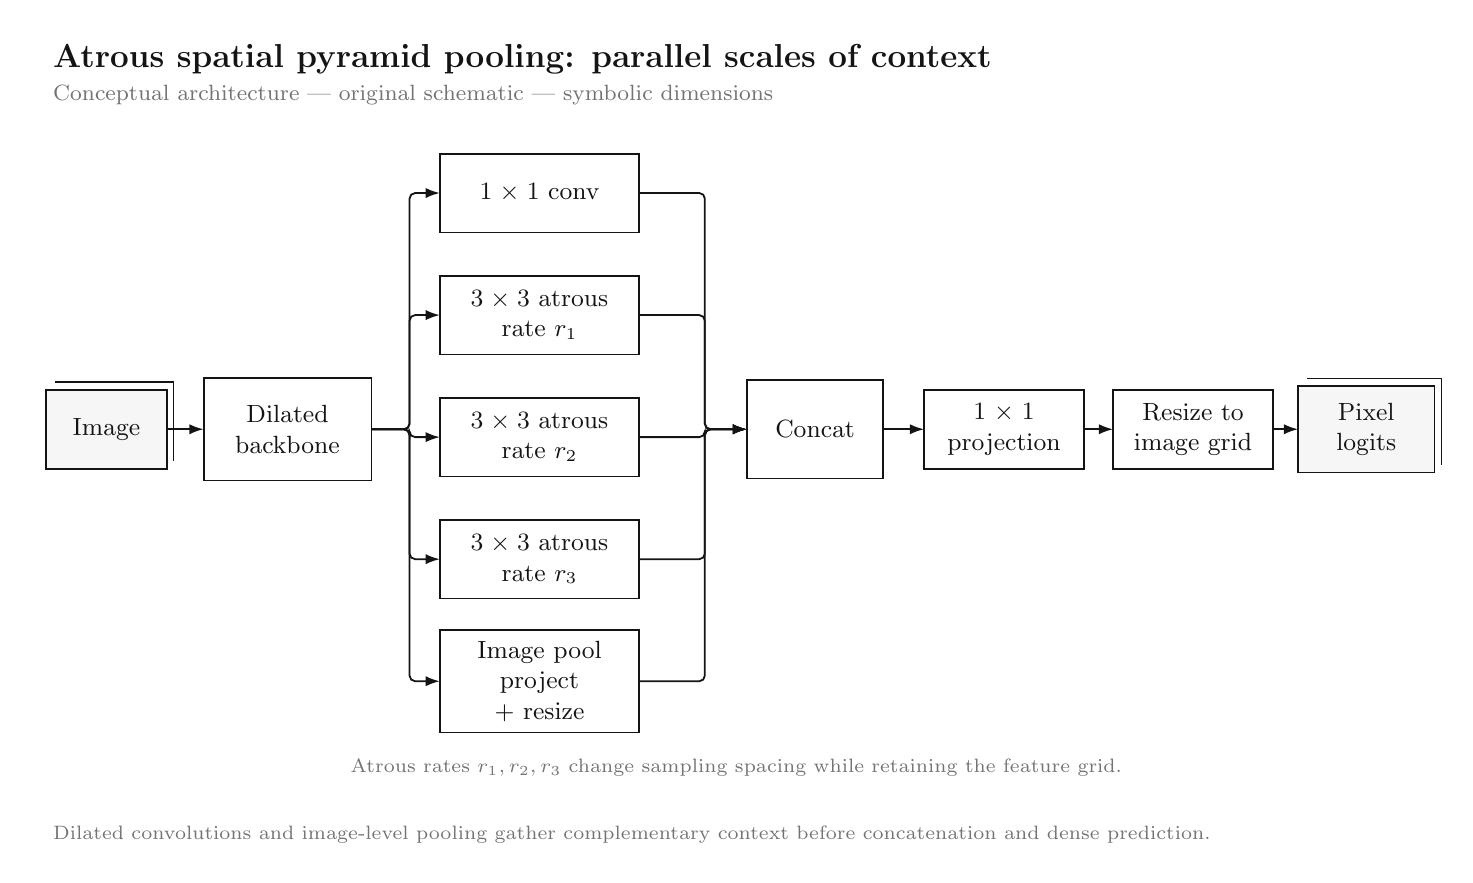
\begin{tikzpicture}[x=1cm,y=-1cm,font=\rmfamily,text=ink]

\path[use as bounding box] (0,0) rectangle (18,10.5);
\node[anchor=west,font=\large\bfseries] at (.2,.4) {Atrous spatial pyramid pooling: parallel scales of context};
\node[anchor=west,font=\footnotesize,text=soft] at (.2,.85) {Conceptual architecture | original schematic | symbolic dimensions};
\begin{pgfonlayer}{background}
\end{pgfonlayer}
\node[box,fill=wash,minimum width=1.5cm,minimum height=1.0cm,text width=1.25cm] (x) at (1.0,5.1) {Image};
\draw[ink,line width=.4pt] (0.35,4.5) -- (1.85,4.5) -- (1.85,5.5);
\node[box,minimum width=2.1cm,minimum height=1.3cm,text width=1.85cm] (back) at (3.3,5.1) {Dilated\\backbone};
\node[box,minimum width=2.5cm,minimum height=1.0cm,text width=2.25cm] (p1) at (6.5,2.1) {$1\times1$ conv};
\node[box,minimum width=2.5cm,minimum height=1.0cm,text width=2.25cm] (a1) at (6.5,3.65) {$3\times3$ atrous\\rate $r_1$};
\node[box,minimum width=2.5cm,minimum height=1.0cm,text width=2.25cm] (a2) at (6.5,5.2) {$3\times3$ atrous\\rate $r_2$};
\node[box,minimum width=2.5cm,minimum height=1.0cm,text width=2.25cm] (a3) at (6.5,6.75) {$3\times3$ atrous\\rate $r_3$};
\node[box,minimum width=2.5cm,minimum height=1.0cm,text width=2.25cm] (pool) at (6.5,8.3) {Image pool\\project + resize};
\node[box,minimum width=1.7cm,minimum height=1.25cm,text width=1.45cm] (cat) at (10.0,5.1) {Concat};
\node[box,minimum width=2.0cm,minimum height=1.0cm,text width=1.75cm] (proj) at (12.4,5.1) {$1\times1$\\projection};
\node[box,minimum width=2.0cm,minimum height=1.0cm,text width=1.75cm] (up) at (14.8,5.1) {Resize to\\image grid};
\node[box,fill=wash,minimum width=1.7cm,minimum height=1.1cm,text width=1.45cm] (seg) at (17.0,5.1) {Pixel\\logits};
\draw[ink,line width=.4pt] (16.25,4.45) -- (17.950000000000003,4.45) -- (17.950000000000003,5.55);
\begin{pgfonlayer}{background}
\draw[flow] (x.east) -- (back.west);
\draw[flow] (back.east) -- (4.85,5.1) -- (4.85,2.1) -- (p1.west);
\draw[flow] (back.east) -- (4.85,5.1) -- (4.85,3.65) -- (a1.west);
\draw[flow] (back.east) -- (4.85,5.1) -- (4.85,5.2) -- (a2.west);
\draw[flow] (back.east) -- (4.85,5.1) -- (4.85,6.75) -- (a3.west);
\draw[flow] (back.east) -- (4.85,5.1) -- (4.85,8.3) -- (pool.west);
\draw[flow] (p1.east) -- (8.6,2.1) -- (8.6,5.1) -- (cat.west);
\draw[flow] (a1.east) -- (8.6,3.65) -- (8.6,5.1) -- (cat.west);
\draw[flow] (a2.east) -- (8.6,5.2) -- (8.6,5.1) -- (cat.west);
\draw[flow] (a3.east) -- (8.6,6.75) -- (8.6,5.1) -- (cat.west);
\draw[flow] (pool.east) -- (8.6,8.3) -- (8.6,5.1) -- (cat.west);
\draw[flow] (cat.east) -- (proj.west);
\draw[flow] (proj.east) -- (up.west);
\draw[flow] (up.east) -- (seg.west);
\end{pgfonlayer}
\node[annotation,text width=15cm] at (9,9.4) {Atrous rates $r_1,r_2,r_3$ change sampling spacing while retaining the feature grid.};
\node[anchor=west,align=left,font=\scriptsize,text=soft,text width=17.6cm] at (.2,10.25) {Dilated convolutions and image-level pooling gather complementary context before concatenation and dense prediction.};
\end{tikzpicture}
\end{document}
